\documentclass[../../note.tex]{subfiles}

\begin{document}

\chapter{Measure Theory}
\section{Sigma algebra}
\begin{example}
    We define $\mathcal{P}(X)$ as the power set of set $X$. Assume that set $X = \left\{a,b\right\}$, the power set $P(X)$ would be $\left\{\emptyset, X, \{a\}, \{b\}\right\}$
\end{example}
\begin{definition}[Sigma algebra]
    $\mathcal{A} \subseteq \mathcal{P}(X)$ is called a $\sigma-{\rm algebra}$:
    \begin{align}
        (a)~& \emptyset, X \in \mathcal{A} \\
        (b)~& A \in \mathcal{A} \Longrightarrow A^c:= X \text{\textbackslash} A \in \mathcal{A} \\
        (c)~& A_i \in \mathcal{A},~i \in \mathcal{N}\Longrightarrow \cup_{i=1}^{\infty} A_i \in \mathcal{A}.
    \end{align}
\end{definition}

\begin{definition}[Measurable sets]
    $A \in \mathcal{A}$ is called a $\mathcal{A}$-measurable set.
\end{definition}

\begin{example}
    \begin{align}
        (1)~&\mathcal{A} = \left\{\emptyset, X \right\} \\
        (2)~&\mathcal{A} = \left\{\mathcal{P}(X)\right\}.
    \end{align}
\end{example}

\begin{lemma}
    Assume $\mathcal{A}_i$ is $\sigma$-algebra on $X$, $i\in I$(index set). Then, we have $\cap_{i \in I} \mathcal{A}_i$ is also a $\sigma$-algebra on $X$.
\end{lemma}

\begin{definition}[Sigma algebra generated by $\mathcal{M}$]
    For $\mathcal{M} \subseteq \mathcal{P}(X)$, there is a smallest $\sigma$-algebra that contains $\mathcal{M}$:
    \begin{align}
        \sigma(\mathcal{M})
        &:= \cap_{\mathcal{A}\supseteq \mathcal{M},~a~\sigma-algebra} \mathcal{A}.
    \end{align}
\end{definition}

\begin{example}
    We define $X = \left\{a,b,c,d\right\}$ and $\mathcal{M}=\left\{\left\{a\right\}, \left\{b\right\}\right\}$. Then we have 
    \begin{align}
        \sigma(\mathcal{M})
        &= \left\{\emptyset, X, \left\{a\right\}, \left\{b\right\},\left\{a,b\right\}, \left\{b,c,d\right\},\left\{a,c,d\right\}, \left\{c,d\right\}\right\}.
    \end{align}
\end{example}

\begin{definition}[Borel sigma algebra]
    Let $(X, \mathcal{T})$ be a topological space (Let $X$ be a metric space/Let $X$ be a subset of $\mathbb{R}^n$; We need "open sets".). We then define $\mathcal{B}(X)$ is the borel $\sigma$-algebra on $X$ as
    \begin{align}
        \mathcal{B}(X)
        &:= \sigma(\mathcal{T}),
    \end{align}
    which is the $\sigma$-algebra generated by the open sets $\mathcal{T}$.
\end{definition}

\section{What is a measure?}
\begin{definition}[Measure]
    $(X, \mathcal{A})$ is called a measurable space, where $X$ is a set and $\mathcal{A}$ is a $\sigma$-algebra on $X$. A map $\mu:~\mathcal{A} \rightarrow [0,\infty]:= [0,\infty)+\left\{\infty\right\}$ is called a measure if it satisfies:
    \begin{align}
        (a)~& \mu(\emptyset) = 0 \\
        (b)~& \mu(\cup_{i=1}^{\infty}\mathcal{A}_i) = \sum_{i=1}^{\infty} \mu(\mathcal{A}_i)~with~\mathcal{A}_i \cap \mathcal{A}_j = \emptyset,~i \neq j~for~all~\mathcal{A}_i \in \mathcal{A}. (\sigma-additive) 
    \end{align}
\end{definition}

\begin{definition}
    $(X,\mathcal{A},\mu)$ is called a measure space.
\end{definition}

\begin{example}
    Given $X$ and $\mathcal{A} = \mathcal{P}(X)$.
    \begin{itemize}
        \item Counting measure ($A \in \mathcal{A}$) is defined as
        \begin{align}
            \mu(A):= \left\{
                \begin{matrix}
                    \#A,&~A~\text{has finitely many elements} \\
                    \infty&~\text{else}
                \end{matrix}
            \right.
        \end{align}
        where $\# A$ means the number of elements in $A$.

        Calculation rules in $[0,\infty]$:
        \begin{align}
            x+\infty&:= \infty~for~all~x\in[0,\infty] \\
            x\cdot \infty&:= \infty~for~all~x\in(0,\infty] \\
            0\cdot \infty&:= 0~(\text{only true in most cases in measure theory!})
        \end{align}
    \item Dirac measure for $p \in X$ is defined as
    \begin{align}
        \delta_{p}(A)
        &:= \left\{
            \begin{matrix}
                1,~& p \in A \\
                0,~& else
            \end{matrix}
        \right.
    \end{align}
    \item We search a measure on $X \in \mathcal{R}^n$ satisfying:
    \begin{align}
        (1)~&\mu([0,1]^n) = 1 \\
        (2)~&\mu(x+A) = \mu(A)~for~all~x\in \mathcal{R}^n,
    \end{align}
    which is known as Lebesgue measure where the $\sigma$-algebra is not equal to power set.
\end{itemize}
\end{example}

\section{Not everything is lebesgue measurable}

\textbf{Measure problem:} search measure $\mu$ on $\mathcal{P}(\mathbb{R})$ with:
\begin{itemize}
    \item (1) $\mu([a, b]) = b - a,~b > a$,
    \item (2) $\mu(x+A) = \mu(A),~A \in \mathcal{P}(\mathbb{R}),~x \in \mathbb{R}$.
\end{itemize}
$\Longrightarrow$ $\mu$ does not exist.

\textbf{Claim:} Let $\mu$ be a measure on $\mathcal{P}(\mathbb{R})$ with $\mu((0, 1])<\infty$ and (2). $\Longrightarrow \mu = 0.$
\begin{proof}
    (a) Definitions: $I \in (0,1]$ with equivalence relation on $I$: $x {\sim} y \Longleftrightarrow x - y \in \mathbb{Q}$ i.e., $[x]:= \left\{x+r \vert r \in \mathbb{Q},~ x+r \in I \right\}$. Following this definition, we have a disjoint decomposition of $I$ into boxes, possibly uncontable many of them! We then pick one element $a_n$ from each box $[x_n]$ and form a set $A \in I$, i.e., $\left\{a_1, a_2, \cdots \right\} = A$. We have $A \in I$ with prperty:
    \begin{itemize}
        \item (1) For each $[x]$, there is an $a \in A$ with $a \in [x]$.
        \item (2) For all $a, b \in A:~a,b \in [x]\Longrightarrow a=b$.
    \end{itemize} 
    In uncountable case, the existence of $A \in I$ with the above property is guaranted by the axiom of choice of set theory.

    We define $A_n:= r_n + A$, where $(r_n)_{n \in \mathbb{N}}$ enumeration of $\mathbb{Q}_n(-1, 1]$. 
    
    (b) We then claim that $A_n \cap A_m = \emptyset \Longleftarrow n \neq m$. The proof is as follows: $x \in A_n \cap A_m$ $\Longrightarrow$ $x= r_n + a_n,~ a_n \in A$ and $x= r_m + a_m,~ a_m \in A$. $\Longrightarrow r_n + a_n = r_m + a_m \Longrightarrow a_n-a_m = r_n-r_m \in \mathbb{Q} \Longrightarrow a_n \sim a_m \Longrightarrow a_m, a_n \in [a_m] \Longrightarrow a_n = a_m \Longrightarrow r_n=r_m \Longrightarrow n=m$.

    (c) We claim that $(0,1] \subseteq \cup_{n \in \mathbb{N}} A_n \subseteq (-1, 2]$. The proof is as follows:

    Assume now: $\mu$ measure on $\mathcal{P}(\mathbb{R})$ with $\mu ((0,1])< \infty $ and (2).

    By (2): $\mu(1+A) = \mu(A)$ for all $n \in \mathbb{N}$.

    By (c): 
    we have 
    \begin{align}
        \label{measure problem (c)}
        \mu((0,1]) \leq \mu(\cup_{n \in \mathbb{N}} A_n) \leq \mu((-1,2])
    \end{align}
    We know: $\mu((0,1]) =: C < \infty $. By using (2) and $\sigma$-additivity, we get $\mu((-1,2]) = \mu\left((-1,0] \cup (0,1] \cup (1,2] = 3 C\right)$. $\Longrightarrow_{\ref{measure problem (c)}, (b)} C \leq \sum_{n=1}^{\infty} \mu(A_n) \leq 3 C \Longrightarrow C \leq \sum_{n=1}^{\infty} \mu(A) \leq 3 C \Longrightarrow \mu(A) = 0 \Longrightarrow C=0$(henceL $\mu\left((0,1]\right)=0$) $\Longrightarrow \mu(\mathbb{R}) = \mu\left(\cup_{n \in \mathbb{Z}}(m,m+1]\right) = 0 \Longrightarrow \mu = 0$. 
\end{proof}

\section{Measurable maps}
\begin{definition}[Measurable maps]
    $(\Omega_1, \mathcal{A}_1)$ and $(\Omega_2, \mathcal{A}_2)$ are measurable spaces. $f: \Omega_1 \rightarrow \Omega_2$ is a measurable map w.r.t. $\mathcal{A}_1$ and $\mathcal{A}_2$  if $f^{-1}(A_2) \in \mathcal{A}_1$ for all $A_2 \in \mathcal{A}_2$.
\end{definition}

\begin{example}
    \begin{itemize}
        \item $(\Omega, \mathcal{A})$ and $(\mathbb{R}, \mathcal{B}(\mathbb{R}))$ are two measurable spaces. We define characteristic fucntion (aksi indicator function) as $\chi_{A}:\Omega \rightarrow \mathbb{R}$, where
        \begin{align}
            \chi_{A}(w)
            &:= \left\{
                \begin{matrix}
                    1,~& w \in A \\
                    0,~& w \notin A
                \end{matrix}
            \right.
        \end{align}
        For all measurable $A \in \mathcal{A}$, $\chi_A$ is a measurable map. We have
        \begin{align}
            \chi_A^{-1}(\emptyset) 
            &= \emptyset \in \mathcal{A},~ \chi_A^{-1}(\mathbb{R}) = \Omega \in \mathcal{A} \\
            \chi_A^{-1}(\left\{\textcolor{red}{A}\right\}) 
            &= A,~ \chi_A^{-1}(\left\{0\right\}) = A^c \in \mathcal{A}.
        \end{align}
        \item Composition of measurable maps. 
        \begin{lemma}
            $(\Omega_1, \mathcal{A}_1),~(\Omega_2, \mathcal{A}_2),~(\Omega_3, \mathcal{A}_3)$ are measurable space. We define $\Omega_1 \stackrel{f}{\rightarrow}\Omega_2 \stackrel{g}{\rightarrow} \Omega_3$. Then $f,g$ are measurable implies $g \circ f$ is measurable.
        \end{lemma}
        \begin{proof}
            \begin{align}
                (g \circ f)^{-1}(A_3)
                &= f^{-1}(g^{-1}(A_3)) \\
                &\in \mathcal{A}_1
            \end{align}
        \end{proof}
    \end{itemize}
\end{example}

\paragraph{Important measurable maps}
\begin{lemma}
    $(\Omega,\mathcal{A})$ and $(\mathbb{R}, \mathcal{B}(\mathbb{R}))$ are measurable spaces. $f,g: \Omega \rightarrow \mathbb{R}$ are measurable maps indicates that $f+g,~f-g,~f \cdot g,~\vert f \vert$ are measurable maps.
\end{lemma}

\section{Lebesgue integral}
\begin{example}
    Define Characteristic function $\chi_A: X \rightarrow \mathbb{R},~A \in \mathcal{A}$. We define $I(A):= \mu(A)$. Surprisingly, $I(A)$ is nothing but the integral of $\chi_A$ over $A$.
\end{example}

\begin{definition}[Simple/Step/Staircsae functions,\dots]
    \label{simple functions}
    For $A_1, A_2,\dots, A_n \in \mathcal{A},$ and $~c_1,c_2, \cdots, c_n \in \mathbb{R}$. We define
    \begin{align}
        f(x)
        &:= \sum_{i=1}^n c_i \cdot \chi_{A_i}(x).
    \end{align}
    We then have $f(x)$ is measurable and the integraal of $f$ is defined as $I(f):= \sum_{i=1}^n c_i \mu(A_i)$.
\end{definition}
\begin{remark}
    The problem of the integral $I(f)$ is that it is undefined when $\mu(A_i) = \infty$. The problem can be solved by exclude $\infty$ by defintion or the following way.
\end{remark}

\begin{definition}[Lebesgue integral]
    Define $S^+:= \left\{f:X\rightarrow\mathbb{R} \vert f~simple~function,~f \geq 0\right\}$. $f \in S^+$ and choose representation $f(x) = \sum_{i=1}^n c_i \chi_{A_i}(x),~c_i \geq 0$. The lebesgue integral of $f$ w.r.t. $\mu$ is defined as
    \begin{align}
        \int_X f(x)~{\rm d}\mu(x) 
        &= \int_X f~{\rm d}\mu \\
        &= I(f) \\
        &= \sum_{i=1}^n c_i \cdot \mu(A_i) \\
        &= [0,\infty].
    \end{align}
\end{definition}

\begin{property}
    \begin{itemize}
        \item $I(\alpha f + \beta g) = \alpha I(f) + \beta I(g),~\alpha,\beta \geq 0$.
        \item $f \leq g \Longrightarrow I(f) \leq I(g)$ (monotomicity)
    \end{itemize}
\end{property}

\begin{definition}
    Define  a measurable map $f: X \rightarrow [0,\infty)$. $h = \sum_{i=1}^{n} c_i \cdot \chi_{A_i}$. The lebesgue integral of $f$ w.r.t. $\mu$ is defined as
    \begin{align}
        \int_X f~{\rm d}\mu
        &:= \sup\left\{I(h) \vert h \in S^
        +,~h \leq f \right\} \\
        & \in [0, \infty].
    \end{align}
    $f$ is called $\mu$-integrable if $\int_X f~{\rm d}\mu < \infty$.
\end{definition}

\begin{property}
    \label{property of lebesgue integral}
    Define measurable maps $f,g: X \rightarrow [0,\infty)$, we have
    \begin{itemize}
        \item 1. $f=g$ for $\mu$-almost everywhere(a.e.), which satisfies $\mu\left(\left\{x \in X \vert f(x) \neq g(x) \right\}\right)=$ $\Longrightarrow \int_X f~{\rm d}\mu = \int_X g~{\rm d}\mu$.
        \item 2. $f \leq g$ for $\mu$ a.e. $\Longrightarrow \int_X f~{\rm d}\mu \leq \int_X g~{\rm d}\mu$
        \item 3. $f=0$ for $\mu$-a.e. $\Longleftrightarrow$ $\int_X f~{\rm d}\mu = 0$.
    \end{itemize}
\end{property}
\begin{proof}[Proof of 2.: monotonicity]
    Let $h:= X \rightarrow [0,\infty)$ be a simple function, i.e.,
    \begin{align}
        h(x) 
        &= \sum_{i=1}^n c_i \chi_{A_i}(x) \\
        &= \sum_{t \in h(X)} t \cdot \chi_{\left\{x \in X \vert h(x) = t \right\}}.
    \end{align}
    Let $X = \tilde{X}^c \cup \tilde{X}$ with $\mu(\tilde{X}^c) = 0$,
    \begin{align}
        \tilde{h}(x)
        &:= \left\{
            \begin{matrix}
                h(x),~&x \in \tilde{X} \\
                a,~&x \in \tilde{X}^c
            \end{matrix}
        \right. \\
        \tilde{h}(x)
        &= \sum_{t \in h(X)} t \cdot \chi_{\left\{x \in \tilde{X} \vert h(x) = t \right\}} + a \cdot \chi_{\tilde{X}^c} \\
        I(\tilde{h})
        &= \sum_{t \in h(X)} t \cdot \mu(\left\{x \in \tilde{X} \vert h(x) = t \right\}) + a \cdot \mu(\tilde{X}^c) \\
        &= \sum_{t \in h(X)} t \left[\mu\left(\left\{x \in \tilde{X} \vert h(x) = t \right\}\right) + \mu \left(\left\{x \in \tilde{X}^c \vert h(x) = t \right\}\right)\right] \\
        &= \sum_{t \in h(X)} t \left[\mu\left(\left\{x \in \tilde{X} \vert h(x) = t \right\} \cup \left\{x \in \tilde{X}^c \vert h(x) = t \right\}\right)\right] \\
        I(h) 
        &= \sum_{t \in h(X) \mbox{\textbackslash} \left\{0\right\}} t \cdot \mu\left(\left\{x \in X \vert h(x) = t \right\}\right). 
    \end{align}
    We define
    \begin{align}
        \tilde{X}
        &:= \left\{x \in X \vert f(x) \leq g(x) \right\}, \\
        \mu(\tilde{X}^c) 
        &= 0 \\
        \int_X f~{\rm d}\mu 
        &= \sup\left\{I(h) \vert h \in S^+, h \leq f \right\} \\
        &= \sup\{I(\tilde{h})\vert \tilde{h} \in S^+, \tilde{h} \leq f ~on~\tilde{X}\} \\
        &\leq \sup\{I(\tilde{h}) \vert \tilde{h} \in S^+, h \leq g ~on~\tilde{X}\} \\
        &= \sup\{I({h}) \vert {h} \in S^+, h \leq g\} \\
        &= \int_X g~{\rm d}\mu.
    \end{align}
\end{proof}

\begin{theorem}[Monotone convergence theorem]
    \label{thm: monotone convergence theorem}
    $(X, \mathcal{A}, \mu)$ measurable spaces, $f_n: X \rightarrow [0,\infty]$, ($f: X \rightarrow [0,\infty]$) measurable for all $n \in \mathbb{N}$ with
    \begin{align}
        &f_1 \leq f_2 \leq f_3 \leq \cdots~~~\mu-\mbox{a.e.}\\  
        (\lim_{n \rightarrow \infty} \int_X f_n~{\rm d}\mu
        &= \int_X f~{\rm d}\mu~~~\mu-\mbox{a.e.}(x \in X))
    \end{align}
    This implies that
    \begin{align}
        \lim_{n \rightarrow \infty} \int_X f_n~{\rm d}\mu 
        &= \int_X \lim_{n \rightarrow} f_n~{\rm d}\mu.
        \label{mct *}
    \end{align}
\end{theorem}
\begin{proof}
    $\int_X f_1~{\rm d}\mu \leq \int_X f_2~{\rm d}\mu \leq \cdots$ and $\int_X f_n~{\rm d}\mu \leq \int_X f~{\rm d}\mu$ for $n \in \mathbb{N}$. Then we have
    \begin{align}
        \lim_{n \rightarrow \infty} \int_X f_n~{\rm d}\mu 
        &\leq \int_X f~{\rm d}\mu,
    \end{align}
    which is the first part of \ref{mct *}.

    Let $h$ be a simple function $0 \leq h \leq f$ and $\varepsilon > 0$. We define 
    \begin{align}
        X_n:= \left\{x\in X \vert f_n(x) \geq (1-\varepsilon)h(x) \right\}
    \end{align}
    with $\cup_{n=1}^{\infty} X_n = \tilde{X}$, and $\mu(\tilde{X}^c) = 0$. We have
    \begin{align}
        \int_X f_n~{\rm d}\mu 
        &\geq \int_{X_n} f_n~{\rm d}\mu \geq \int_{X_n} (1-\varepsilon)h~{\rm d}\mu \\
        \lim_{n \rightarrow \infty} \int_X f_n~{\rm d}\mu
        &\geq \lim_{n \rightarrow \infty} \int_{X_n} (1-\varepsilon)h~{\rm d}\mu \\
        &= \int_{\tilde{X}} (1-\varepsilon)h~{\rm d}\mu \\
        &= \int_X (1-\varepsilon)h~{\rm d}\mu.
    \end{align}
    This implies
    \begin{align}
        \lim_{n \rightarrow \infty} \int_X f_n~{\rm d}\mu 
        &\geq \int_X h~{\rm d}\mu,
    \end{align}
    since $\varepsilon > 0$ arbitrarily. Then we have
    \begin{align}
        \lim_{n \rightarrow \infty} \int_X f_n~{\rm d}\mu 
        &\geq \int_X f{\rm d}\mu,
    \end{align}
    since $h$ is arbitrary and $h \leq f$, which is second part of \ref{mct *}.
\end{proof}

\paragraph{Applictions}
    Given a series $(g_n)_{n \in \mathbb{N}}$, $g_n: X \rightarrow [0,\infty]$ measurable for all $n$. Then we have $\sum_{n=1}^\infty g_n: X \rightarrow [0,\infty]$ measurable and 
    \begin{align}
        \int_X \sum_{n=1}^{\infty} g_n~{\rm d}\mu
        &= \sum_{n=1}^{\infty} \int_X g_n~{\rm d}\mu,
    \end{align}
    which means the integral and sum can exchange.

\section{Fatou' lemma}
\begin{lemma}[Fatou' lemma]
    \label{lemma: fatou' lemma}
    Given $(X, \mathcal{A}, \mu)$ measurable space, $f_n: X \rightarrow [0,\infty]$ measurable for all $n \in \mathbb{N}$. Then we have
    \begin{align}
        \int_X \liminf_{n \rightarrow \infty} f_n~{\rm d}\mu
        &\leq \liminf_{n \rightarrow \infty} \int_X f_n~{\rm d}\mu.
    \end{align}
\end{lemma}
\begin{remark}
    $\liminf_{n \rightarrow \infty} f_n: X \rightarrow [0,\infty]$ is a function. This is
    \begin{align}
        g(x)
        &:= \left(\liminf_{n \rightarrow \infty} f_n \right)(x) \\
        &:= \lim_{n \rightarrow \infty} \left(\inf_{k \geq n} f_k(x)\right) \\
        &\in [0,\infty] \\
        g_n(x)
        &:= \inf_{k \geq n} f_k(x).
    \end{align}
    We have 
    \begin{align}
        g_1 \leq g_2 \leq g_3 \leq \cdots ,
    \end{align}
    which is monotonically increasing. All these functions are measurable.
\end{remark}
\begin{proof}
    \begin{align}
        \shortintertext{Since (\ref{thm: monotone convergence theorem}),}
        \int_X \lim_{n \rightarrow \infty}g_n~{\rm d}\mu 
        &= \lim_{n \rightarrow \infty} \int_X g_n~{\rm d}\mu \\
        &= \liminf_{n \rightarrow \infty} \int_X g_n~{\rm d}\mu.
    \end{align}
    We know that $g_n \leq f_n$ for all $n \in \mathbb{N}$. By (\ref{property of lebesgue integral}), we have
    \begin{align}
        \int_X g_n~{\rm d}\mu
        &\leq \int_X f_n~{\rm d}\mu,
    \end{align}
    for all $n \in \mathbb{N}$. Then we have
    \begin{align}
        \int_X \liminf_{n \rightarrow \infty} f_n~{\rm d}\mu
        &= \liminf_{n \rightarrow \infty} \int_X g_n~{\rm d}\mu \\
        &\leq \liminf_{n \rightarrow \infty} \int_X f_n~{\rm d}\mu.
    \end{align}
\end{proof}

\section{Lebesgue's dominated convergence theorem}
$(X, \mathcal{A}, \mu)$, $\mathcal{L}^1:= \left\{f: X \rightarrow \mathbb{R}~measurable \vert \int_X \vert f \vert^1~{\rm d}\mu < \infty \right\}$. For $f \in \mathcal{L}^1(\mu)$, write $f = f^+ - f^-$, where $f^+, f^- \geq 0$. Define $\int_X f~{\rm d}\mu:= \int_X f^+~{\rm d}\mu - \int_X f^-~{\rm d}\mu$.

\begin{theorem}[Lebesgue's dominated convergence theorem]
    \label{thm: lebesgue's dominated convergence theorem}
    $f_n: X \rightarrow \mathbb{R}$ measurable for all $n \in \mathbb{N}$. $f: X \rightarrow \mathbb{R}$ with $\stackrel{n \rightarrow \infty}{f(x)}$ for $x \in X$ ($\mu$-a.e.) and $\vert f_n \vert \leq g$ with $g \in \mathcal{L}^1(\mu)$ for all $n \in \mathbb{N}$, where $g$ is called integral majorant. Then: we have $f_1,f_2,\cdots \in \mathcal{L}^1(\mu)$, $f \in \mathcal{L}^1(\mu)$ and 
    \begin{align}
        \lim_{n \rightarrow \infty} \int_X f_n~{\rm d}\mu
        &= \int_X f~{\rm d}\mu.
    \end{align}
\end{theorem}
\begin{proof}
    \begin{align}
        \vert f_n \vert \leq g
        \stackrel{monotonicity}{\Longrightarrow} 
        &\int_X g~{\rm d}\mu < \infty \\
        \Longrightarrow
        & f_1, f_2, \cdots \in \mathcal{L}^1(\mu) \\
        \vert f \vert \leq g~for~\mu-\mbox{a.e.} \Longrightarrow
        & f \in \mathcal{L}^1(\mu)
    \end{align}
    We will show $\int_X \vert f_n - f \vert~{\rm d}\mu \stackrel{n \rightarrow \infty}{\Longrightarrow} 0$.
    \begin{align}
        \vert f_n -f \vert 
        &\leq \vert f_n \vert + \vert f \vert \leq 2g \\
        &\Longrightarrow h_n:= 2g - \vert f_n -f \vert \geq 0 
        \shortintertext{Hence: $h_n: X \rightarrow [0, \infty]$ measurable for all $n \in \mathbb{N}$. Then by (\ref{lemma: fatou' lemma}),} 
        &\Longrightarrow \int_X \liminf_{n \rightarrow \infty} h_n~{\rm d}\mu \leq \liminf_{n \rightarrow \infty} \int_X h_n~{\rm d}\mu \\
        &\Longrightarrow \int_X 2g~{\rm d}\mu \leq \int_X 2g~{\rm d}\mu - \limsup_{n \rightarrow \infty} \int_X \vert f_n -f \vert~{\rm d}\mu \\
        &\Longrightarrow 0 \leq \liminf_{n \rightarrow \infty} \int_X \vert f_n -f \vert~{\rm d}\mu \leq \limsup_{n \rightarrow \infty} \int_X \vert f_n -f \vert~{\rm d}\mu \leq 0 \\
        &\Longrightarrow \shortintertext{Limits exists and $\lim_{n \rightarrow \infty}\vert f_n -f \vert~{\rm d}\mu = 0$. We conclude that} \\
        &0 \leq \vert \int_X f_n~{\rm d}\mu - \int_X f~{\rm d}\mu \vert = \vert \int_X (f_n-f)~{\rm d}\mu \vert {\leq} \int_X \vert f_n - f \vert~{\rm d}\mu \stackrel{n \rightarrow \infty}{\longrightarrow} 0,
        \shortintertext{where the third inequality is due to the integral's triangle inequality.} \\
        &\Longrightarrow \lim_{n \rightarrow \infty} \int_X f_n~{\rm d}\mu = \int_X f~{\rm d}\mu.
    \end{align}
\end{proof}

\section{Caratheodory's extension theorem}
\begin{theorem}[Caratheodory's extension theorem]
    \label{thm: caratheodory's extension theorem}
$X$ set, $\mathcal{A} \in \mathcal{P}(X)$ semiring of sets. A map $\mu: \mathcal{A} \rightarrow [0, \infty]$. Note that $\mu$ is not a measure, it is called A pre-measure.
\begin{itemize}
    \item Then $\mu$ has an extension $\tilde{\mu}: \sigma(\mathcal{A}) \rightarrow [0, \infty]$, where $\tilde{\mu}$ is a measure and $\sigma(\mathcal{A})$ is a $\sigma$-algebra generated by $\mathcal{A}$, i.e., $\mu(A) = \tilde{\mu}(A)$.
    \item If there is sequence ($S_j$) with $S_j \in \mathcal{A}$, $\cup_{j=1}^{\infty} S_j = X$, then the extension $\tilde{\mu}$ from (a) is unique. ($\tilde{\mu}$ is also $\sigma$-finite)
\end{itemize}
\end{theorem}

\begin{definition}[Semiring set]
    Semiring of sets $\mathcal{A} \subseteq \mathcal{P}(X)$:
    \begin{itemize}
        \item $\emptyset \in \mathcal{A}$ (as for $\sigma$-algebra)
        \item $A,B \in \mathcal{A} \Longrightarrow A \cap B \in \mathcal{A}$
        \item For $A,B \in \mathcal{A}$, there are pairwise disjoint sets $S_1, S_2,\dots, S_n \in \mathcal{A}: \cup_{j=1}^n S_j =  A \backslash B$ 
    \end{itemize}
\end{definition}

\begin{example}
    $A:= \left\{[a,b) \vert a,b \in \mathbb{R}, a\leq b\right\}$ not a $\sigma$-algebra because $\mathbb{R} \notin \mathcal{A}$. But $\sigma(\mathcal{A}) = \mathcal{B}(\mathbb{R})$ (Borel $\sigma$-algebra). Check that $\mathcal{A}$ is semiring set:
    \begin{itemize}
        \item $\emptyset \in \mathcal{A}$ 
        \item 
        \begin{align}
            [a,b) \cap [c,d) 
            &= \left\{
                \begin{matrix}
                    \emptyset,&~b \leq c, d \leq a \\
                    [c,b),&~c \in [a,b), d \notin[a,b) \\
                    \cdots &
                \end{matrix}
            \right.
        \end{align}
        \item         
        \begin{align}
            [a,b) \backslash [c,d) 
            &= \left\{
                \begin{matrix}
                    [a,b),&~d \leq a, b \leq c \\
                    [a,c),&~c \in [a,b), d \notin[a,b) \\
                    [a,c) \cup [d,b),&~c>a, d<b \\
                    \cdots &
                \end{matrix}
            \right.
        \end{align}
    \end{itemize}
\end{example}

\begin{definition}[Pre-measure]
    $\mu: \mathcal{A} \rightarrow [0,\infty]$ with $\mathcal{A}$ semiring os sets:
    \begin{itemize}
        \item $\mu(\emptyset) = 0$
        \item $\mu(\cup_{j=1}^{\infty}) = \sum_{j=1}^{\infty} \mu(A_j)$, for $A_j \in \mathcal{A}$, $A_i \cap A_j = \emptyset$ for $i \neq j$ and $\cup_{j=1}^{\infty} A_j \in \mathcal{A}$.
    \end{itemize}
\end{definition}

\paragraph{Application:}
$A:= \left\{[a,b) \vert a,b \in \mathbb{R}, a\leq b\right\}$, $\mu: \mathcal{A} \rightarrow [0,\infty]$, $\mu([a,b)) = b - a$ is a pre-measure (We can check by the definition of pre-measure). Then by (\ref{thm: caratheodory's extension theorem}), there is a unique extension to $\mathcal{B}(\mathbb{R}) \Longrightarrow$ lebesgue measure.

\section{Lebesgue-Stieltjes measures}
$F: \mathbb{R} \rightarrow \mathbb{R}$ monotonically increasing (non-decreasing).$[a, b)$ is the length of the interval. Now we consider new kinds of intervals:
\begin{align}
    F(b^-) - F(a^-)
    &=: \mu_F([a, b)),
\end{align}
where $F(a^-):= \lim_{\varepsilon \rightarrow 0^+} F(a - \varepsilon)$. Alternatively, we also have 
\begin{align}
    F(b^+) - F(a^+)
    &=: \mu_F((a, b]),
\end{align}
where $F(a^+):= \lim_{\varepsilon \rightarrow 0^+} F(a + \varepsilon)$. We consider the previous one hereafter.

\begin{definition}
    $\mathcal{A}:= \left\{[a,b): a,b \in \mathbb{R}, a \leq b \right\}$ semiring of sets. Then by Caratheodory' theorem, we have that there exists exactly one measure
    \begin{align}
        \mu_F: \mathcal{B}(\mathbb{R}) \rightarrow [0, \infty]
        \shortintertext{with $\mu_F([a, b))$}.
    \end{align}
\end{definition}

\begin{example}
    \begin{itemize}
        \item $F(x) = x$, $\mu_F([a, b)) = b - a \rightarrow $ Lebesgue measure.
        \item $F(x) = 1$, $\mu_F([a, b)) = 0 \rightarrow$ zero measure.
        \item 
        \begin{align}
            F(x)
            &= \left\{
                \begin{matrix}
                    0,~& x < 0 \\
                    1,~& x \geq 0
                \end{matrix}
            \right.
        \end{align}
        $\mu_F([-\varepsilon, \varepsilon)) = 1 \rightarrow$ Dirac measure $\delta_0$.
        \item $F: \mathbb{R} \rightarrow \mathbb{R}$ monotonically increasing  + continuously differentiable. Then we have
        \begin{align}
            F': \mathbb{R} \rightarrow [0, \infty)
        \end{align}
        and 
        \begin{align}
            \mu_F([a,b))
            &= F(b) - F(a) \\
            &= \int_a^b F'(x)~{\rm d}x,
        \end{align}
        which implies 
        \begin{align}
            \mu_F: A \longmapsto \int_A F'(x)~{\rm d}x,
        \end{align}
        where $F'(x)$ is called the density function.
    \end{itemize}
\end{example}

\section{Radon-Nikodym theorem and Lebesgue's decomposition theorem}
$(X, \mathcal{A}, \lambda)$ measure space. Special case: $X = \mathcal{R}$, $\mathcal{A} = \mathcal{B}(\mathbb{R})$, and $\lambda$ is lebesgue measure. Recall that $\lambda([a,b)) = b - a$.  Another measure $\mu: \mathcal{B}(\mathbb{R}) \rightarrow [0, \infty]$. We will look how $\mu$ acts w.r.t. the given reference measure: lebesgue measure.

\begin{definition}
    \begin{itemize}
        \item $\mu$ is called absolutely continuous (w.r.t. $\lambda$) if $\lambda(A) = 0 \Longrightarrow \mu(A) = 0$ for all $A \in \mathcal{B}(\mathbb{R})$. One writes: $\mu << \lambda$.
        \item $\mu$ is called singular (w.r.t. $\lambda$) if there is $N \in \mathcal{B}(\mathbb{R})$ with $\lambda(N) = 0$ and $\mu(N^c) = 0$. One writes: $\mu \perp \lambda$.
        \begin{example}
            $\delta_0$ Dirac measure ($\delta_0(\left\{0\right\}) = 1$) $\Longrightarrow \delta_0 \perp \lambda$ (Choose $N = \left\{ 0 \right\}$).
        \end{example}
    \end{itemize}
\end{definition}

\begin{theorem}[Lebesgue's decomposition theorem]
    $\mu: \mathcal{B}(\mathbb{R}) \rightarrow [0, \infty]$ ($\sigma$-finite)
    \begin{itemize}
        \item There are measures (uniquely determined) $\mu_{ac}, \mu_s: \mathcal{B}(\mathbb{R}) \rightarrow [0, \infty]$ with $\mu = \mu_{ac} + \mu_s$, $\mu_{ac} << \lambda, \mu_s \perp \lambda$.
    \end{itemize}
\end{theorem}

\begin{theorem}[Radon-Nikodym theorem]
    $\mu: \mathcal{B}(\mathbb{R}) \rightarrow [0, \infty]$ ($\sigma$-finite)
    \begin{itemize}
        \item There is a measurable map $h: \mathbb{R} \rightarrow [0, \infty)$ with $\mu_{ac} = \int_A d~{\rm d} \lambda$ for all $A \in \mathcal{B}(\mathbb{R})$, where $h$ is called the density function.
    \end{itemize}
\end{theorem}

\section{Image measure and substitution formula}
Image measure is also called pushforward measure. Substitution formula is also called change of variable.

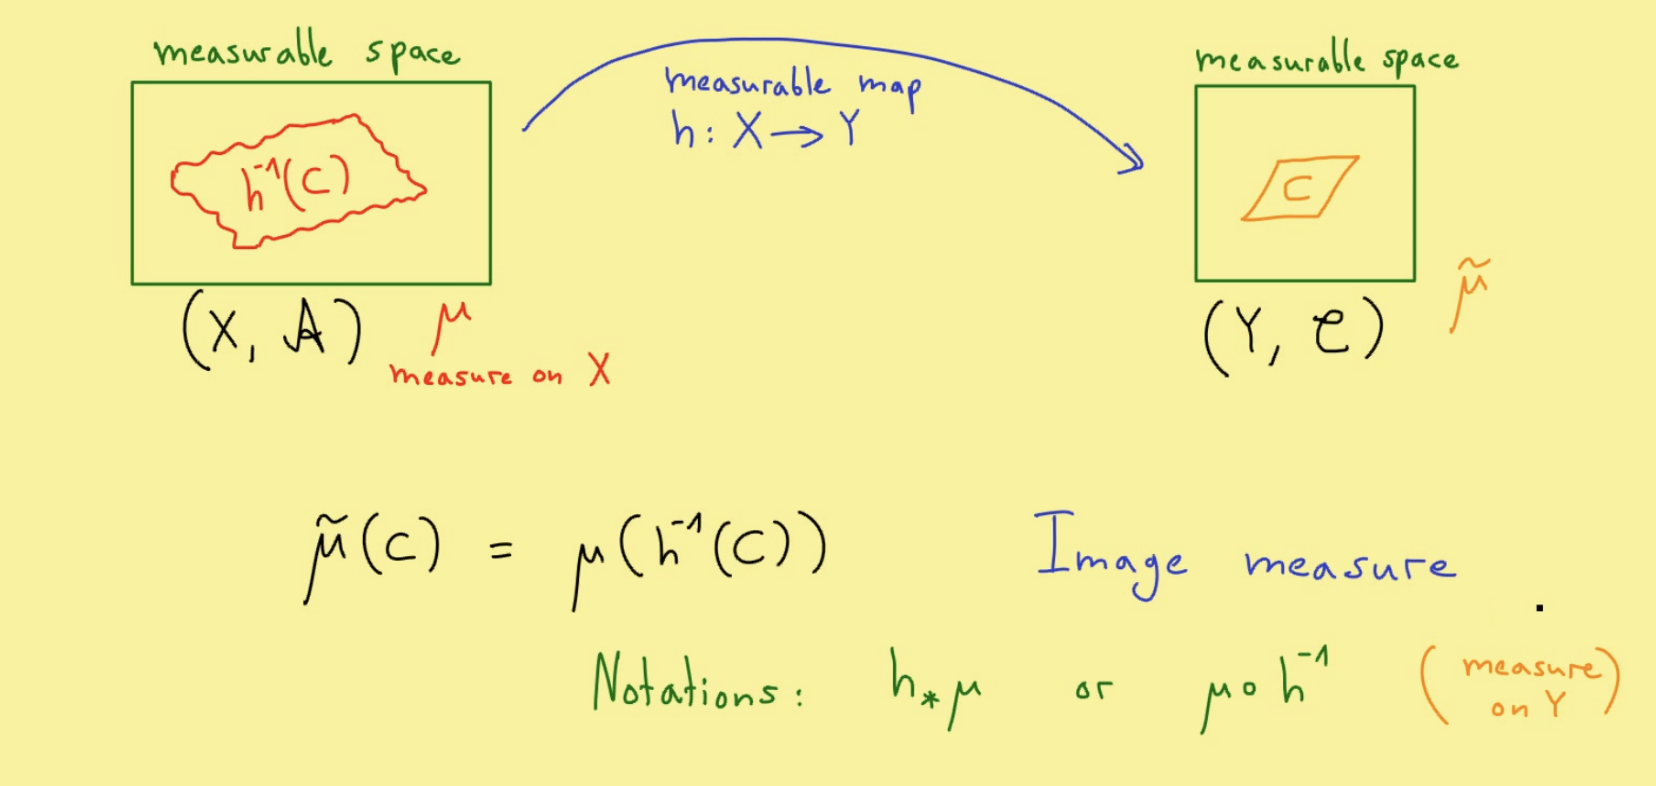
\includegraphics[scale=0.4]{Image measure.png}

\begin{definition}[Image measure]
    Measure space $(X, \mathcal{A})$, $\mu$ is a measure on $X$. Measure space $(Y, \mathcal{E})$, $\tilde{\mu}$ is a measure on $Y$. Define a measure map $h: X \rightarrow Y$. See the above figure. We then define the image measure as
    \begin{align}
        \tilde{\mu}(c)
        &= \mu(h^{-1}(c)).
    \end{align}
    The notations: $h * \mu$ or $\mu \circ h^{-1}$. $h * \mu$ means pushforward and $\mu \circ h^{-1}$ is readble. Remember that $\tilde{\mu}$ is aa measure on $Y$.    
\end{definition}

\begin{lemma}[Substitution formula]
    \label{lemma: substitution formula}
    A integrable function $g: Y \rightarrow \mathbb{R}$. We have 
    \begin{align}
        \int_Y g~{\rm d}(h * \mu) 
        &= \int_X g \circ h~{\rm d}\mu,
    \end{align}
    which can also be written as
    \begin{align}
        \int_Y g(y)~{\rm d}(\mu \circ h^{-1})(y) 
        &= \int_X g(h(x))~{\rm d}\mu(x),
    \end{align}
    which is called the change of variables: $y = h(x)$.
\end{lemma}

\begin{example}
    $F$ is a strictly monotonically increasing and continuously differentiable and surjective function from $(\mathbb{R}, \mathcal{B}(\mathbb{R}))$ with $\mu_F$ as $\mu_F(A) = \int_A F'(x)~{\rm d}x$ to $(\mathbb{R}, \mathcal{B}(\mathbb{R}))$. We have
    \begin{align}
        (F * \mu_F)([a,b))
        &= \mu_F(F^{-1}([a,b))) \\
        &= \mu_F([F^{-1}(a), F^{-1}(b)]) \\
        &= \int_{F^{-1}(a)}^{F^{-1}(b)} F'(x)~{\rm d}x \\
        &= \int_a^b {\rm d}y \\
        &= \lambda([a,b)) \\
        &\Longrightarrow F_x \mu_F = \lambda,
    \end{align}
    Substitution formula:
    \begin{align}
        \int_Y g~{\rm d}(F * \mu_F)
        &= \int_X g \circ F~{\rm d}\mu_F \\
        \Longrightarrow \int_{\mathbb{R}} g(y)~{\rm d}y 
        &= \int_{\mathbb{R}} g(F(x)) F'(x)~{\rm d}x.
    \end{align}
\end{example}

\begin{proof}
    \label{pf of substitution rule}
    (1) Let $g = \chi_c$ with $C \subseteq Y$ measurable. For the left hand side, we have
    \begin{align}
        \int_Y \chi_c~{\rm d}(h * \mu) 
        &= (h * \mu)(c) \\
        &= \mu(h^{-1}(c)).
    \end{align}
    For the right hand side, we have
    \begin{align}
        \int_X \chi_c \circ h~{\rm d}\mu
        &= \int_X \chi_c \circ h~{\rm d}\mu \\
        &= \int_X \chi_c(h(x))~{\rm d}\mu(x) \\
        &= \int_X \chi_{h^{-1}(c)}~{\rm d}\mu \\
        &= \mu(h^{-1}(c)),
    \end{align}
    where
    \begin{align}
        \chi_c(h(x))
        &=\left\{
            \begin{matrix}
                1,~x \in h^{-1}(c) \\
                0,~x \notin h^{-1}(c)
            \end{matrix}
        \right.
    \end{align}
    (2) Let $g$ be a simple function, i.e.,$g = \sum_{i=1}^n \chi_{c_i}$. We then obtatin
    \begin{align}
        \int_Y \sum_{i=1}^n \lambda_i \chi_{c_i}~{\rm d}(h*\mu)
        &= \sum_{i=1}^{n} \lambda_i \int_Y \chi_{c_i}~{\rm d}(h * \mu) \\
        &\qquad\eqnote{By (1)} \nonumber \\
        &= \sum_{i=1}^{n} \lambda_i \int_X \chi_{c_i}(h(x))~{\rm d}\mu(x) \\
        &= \int_X(\sum_{i=1}^n \lambda_i \chi_{c_i})(h(x))~{\rm d}\mu(x) \\
        &= \int_X g \circ h~{\rm d}\mu.
    \end{align}
    (3) Let $g: Y \rightarrow [0,\infty)$ measurable. We have
    \begin{align}
        \int_Y g~{\rm d}(h * \mu) 
        &= \sup\left\{\int_Y \tilde{s}~{\rm d}(h * \mu) \vert \tilde{s}: Y \rightarrow [0,\infty)~simple,~\tilde{s}\leq g\right\}.
    \end{align}
    We have the following equivalence relation:
    \begin{align}
        &\forall y \in h(x): \tilde{s}(y) \leq g(y) \\
        &\Longleftrightarrow \forall x \in X: \tilde{s}(h(x)) \leq g(h(x)) \\
        &[i.e., \tilde{s} \circ h \leq (g \circ h)(x)].
    \end{align}
    Then we have
    \begin{align}
        \int_Y g~{\rm d}(h * \mu) 
        &= \sup\left\{\int_X \tilde{s}\circ~{\rm d}\mu \vert \tilde{s}: Y \rightarrow [0,\infty)~simple,\tilde{s} \circ h \leq g \circ h\right\} \\
        &\qquad\eqnote{Left as exercise} \nonumber \\
        &= \sup\left\{\int_X {s}\circ~{\rm d}\mu \vert {s}: X \rightarrow [0,\infty)~simple,{s} \circ h \leq g \circ h\right\} \\
        &= \int_X g \circ h~{\rm d}\mu.
    \end{align}
\end{proof}

\section{Product measure and Cavalieri's principle}
$(X_1,\mathcal{A}_1,\mu_1)$ measure space and $(X_2,\mathcal{A}_2,\mu_2)$ measure space,
\begin{align}
    \Longrightarrow (X_1 \times X_2, \mathcal{A}, \mu),~where~\mu~is~the~product~measure.
\end{align}
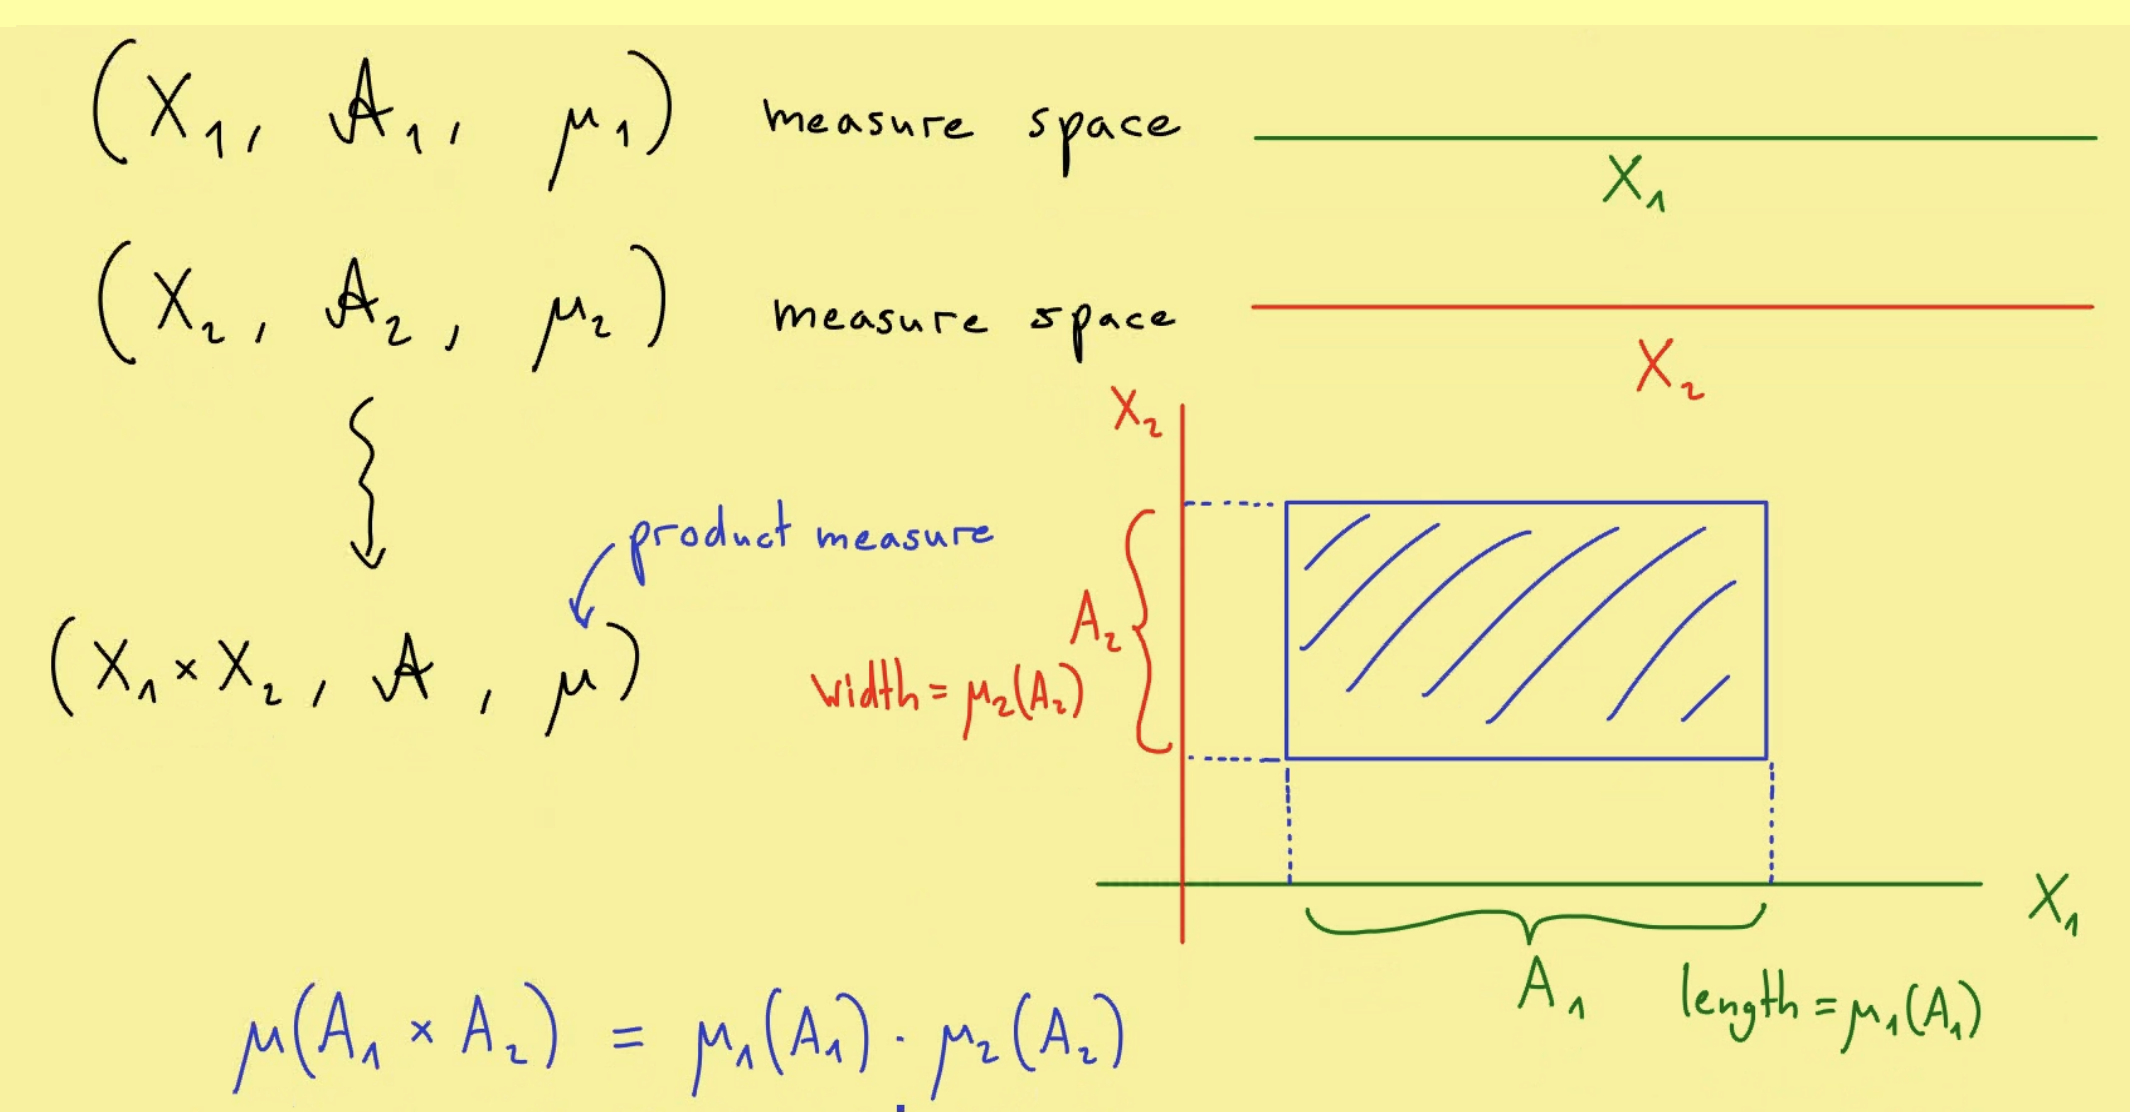
\includegraphics[scale=0.4]{../figures/Product measure.png}
We have
\begin{align}
    \mu(A_1 \times A_2)
    &= \mu_1(A_1) \cdot \mu_2(A_2).
\end{align}
\begin{definition}[Product $\sigma$-algebra]
    \label{Product sigma-algebra}
    \begin{align}
        \mathcal{A}
        &= \sigma(\mathcal{A}_1 \times \mathcal{A}_2).
    \end{align}    
\end{definition}
\begin{remark}
    Set of rectangles (=$\mathcal{A}_1 \times \mathcal{A}_2$) are not a $\sigma$-algebra (but a semiring of sets)
\end{remark}

\begin{definition}
    Define product measure $\mu$ as $\mu(A_1 \times A_2) = \mu_1(A_1) \times \mu_2(A_2)$ for all $A_1 \in \mathcal{A}_1$ and $A_2 \in \mathcal{A}_2$, and use (\ref{thm: caratheodory's extension theorem}).
\end{definition}
\begin{remark}
    Product measure in general not unique.
\end{remark}

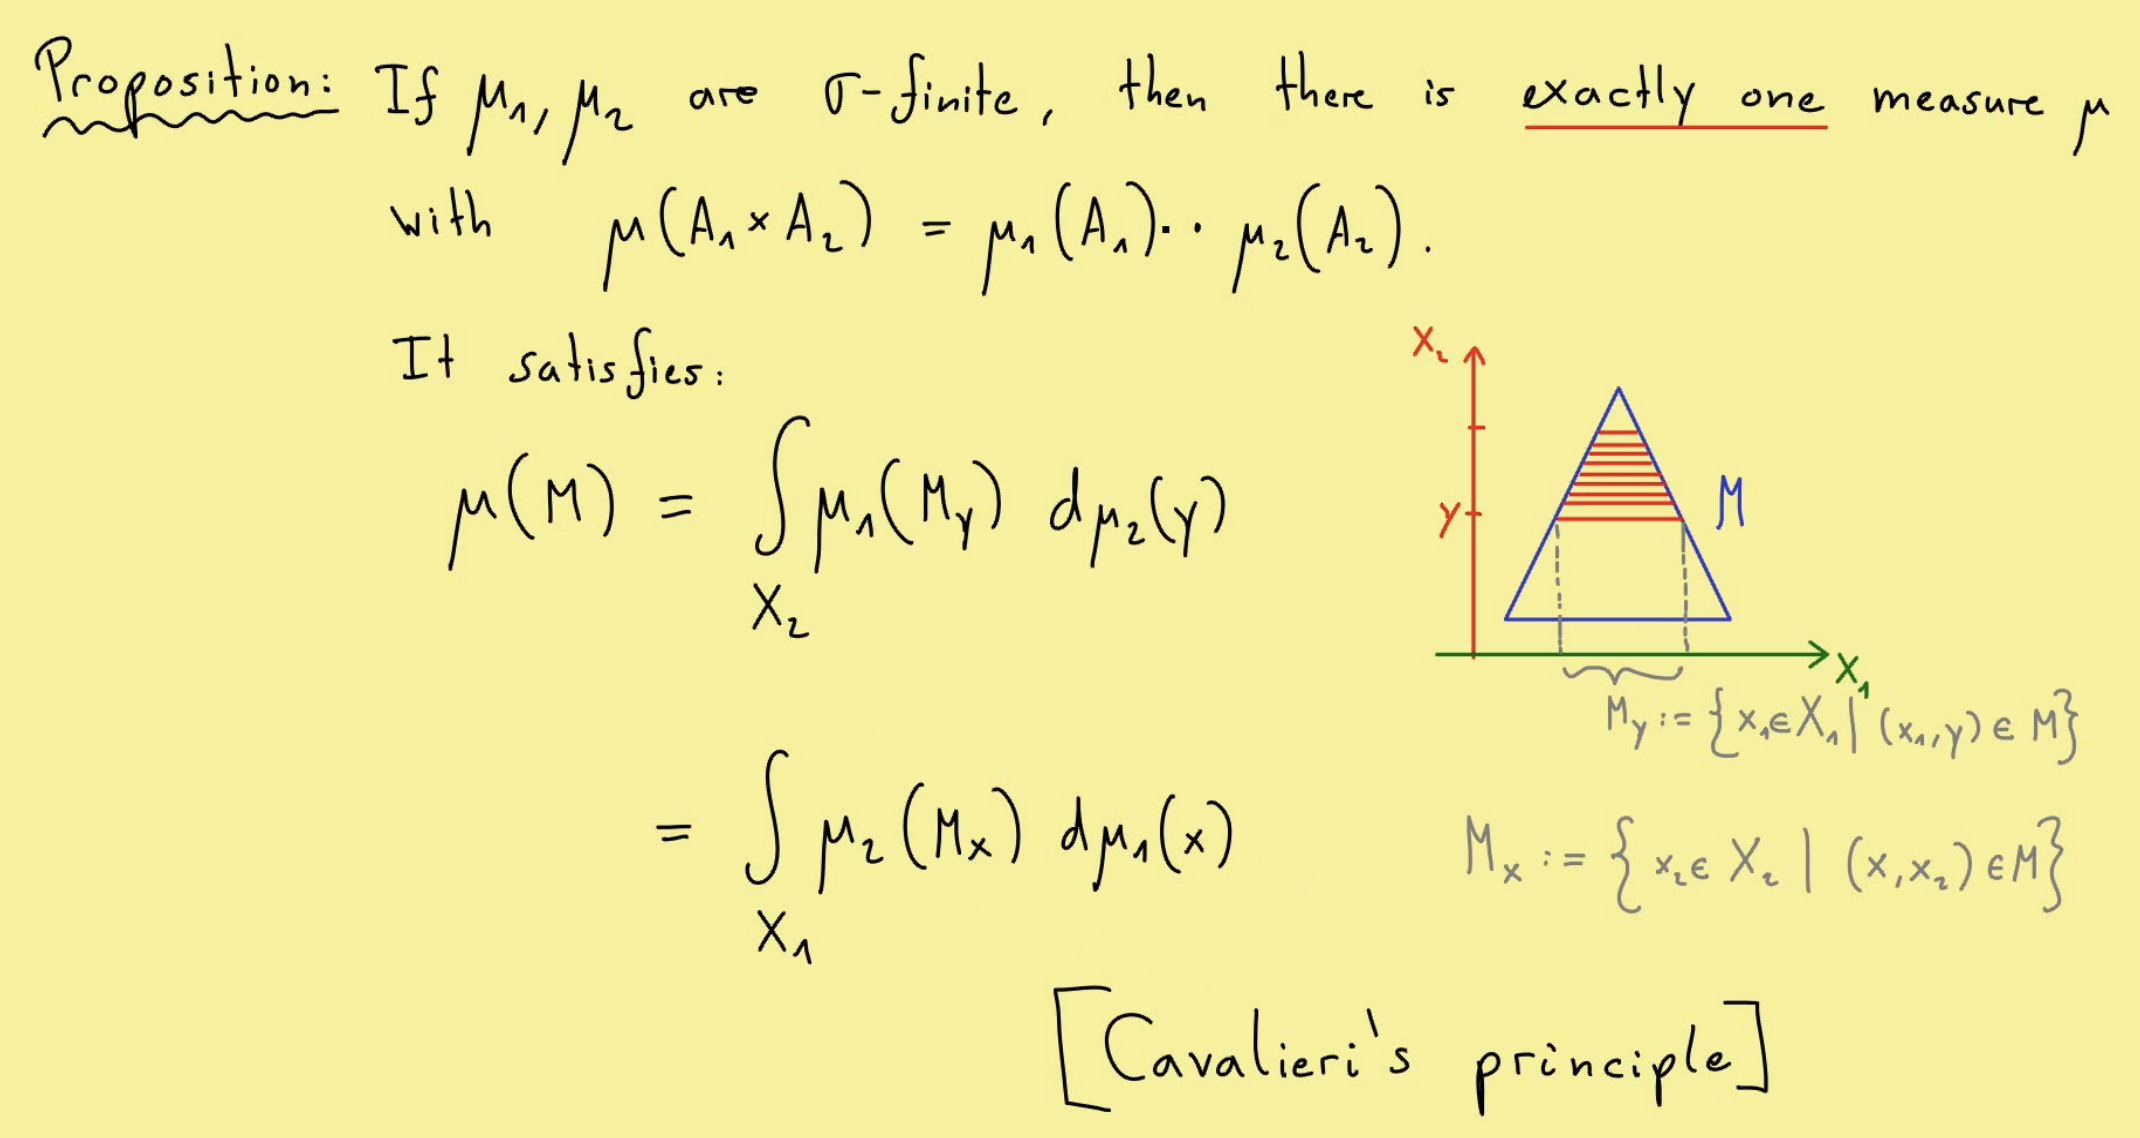
\includegraphics[scale=0.30]{../figures/Cavalieri's principle.png}
\begin{proposition}[Cavalieri's principle]
    \label{thm: cavalieri's principle}
    If $\mu_1$, $\mu_2$ are $\sigma$-finite, then there is exactly one measure $\mu$ with $\mu(A_1 \times A_2)=\mu_1(A_1) \cdot \mu_2(A_2)$. Is satisfies:
    \begin{align}
        \mu(M)
        &= \int_{X_2} \mu_1(M_y)~{\rm d}\mu_2(y) \\
        &= \int_{X_1} \mu_2(M_x)~{\rm d}\mu_1(x).
    \end{align}
\end{proposition}

\begin{example}[An example for Cavalieri's principle]
    Calculate the volume of the pyramid with corners 
    (-1,-1,0), (-1,1,0),(1,-1,0),(1,1,0),(0,0,1), $K \subset \mathbb{R}^3 $, where the volume if the lebesgue measure in $\mathbb{R}^3: \mu$(Recall product measure construction with lebesgus measure on $\mathbb{R}$).

    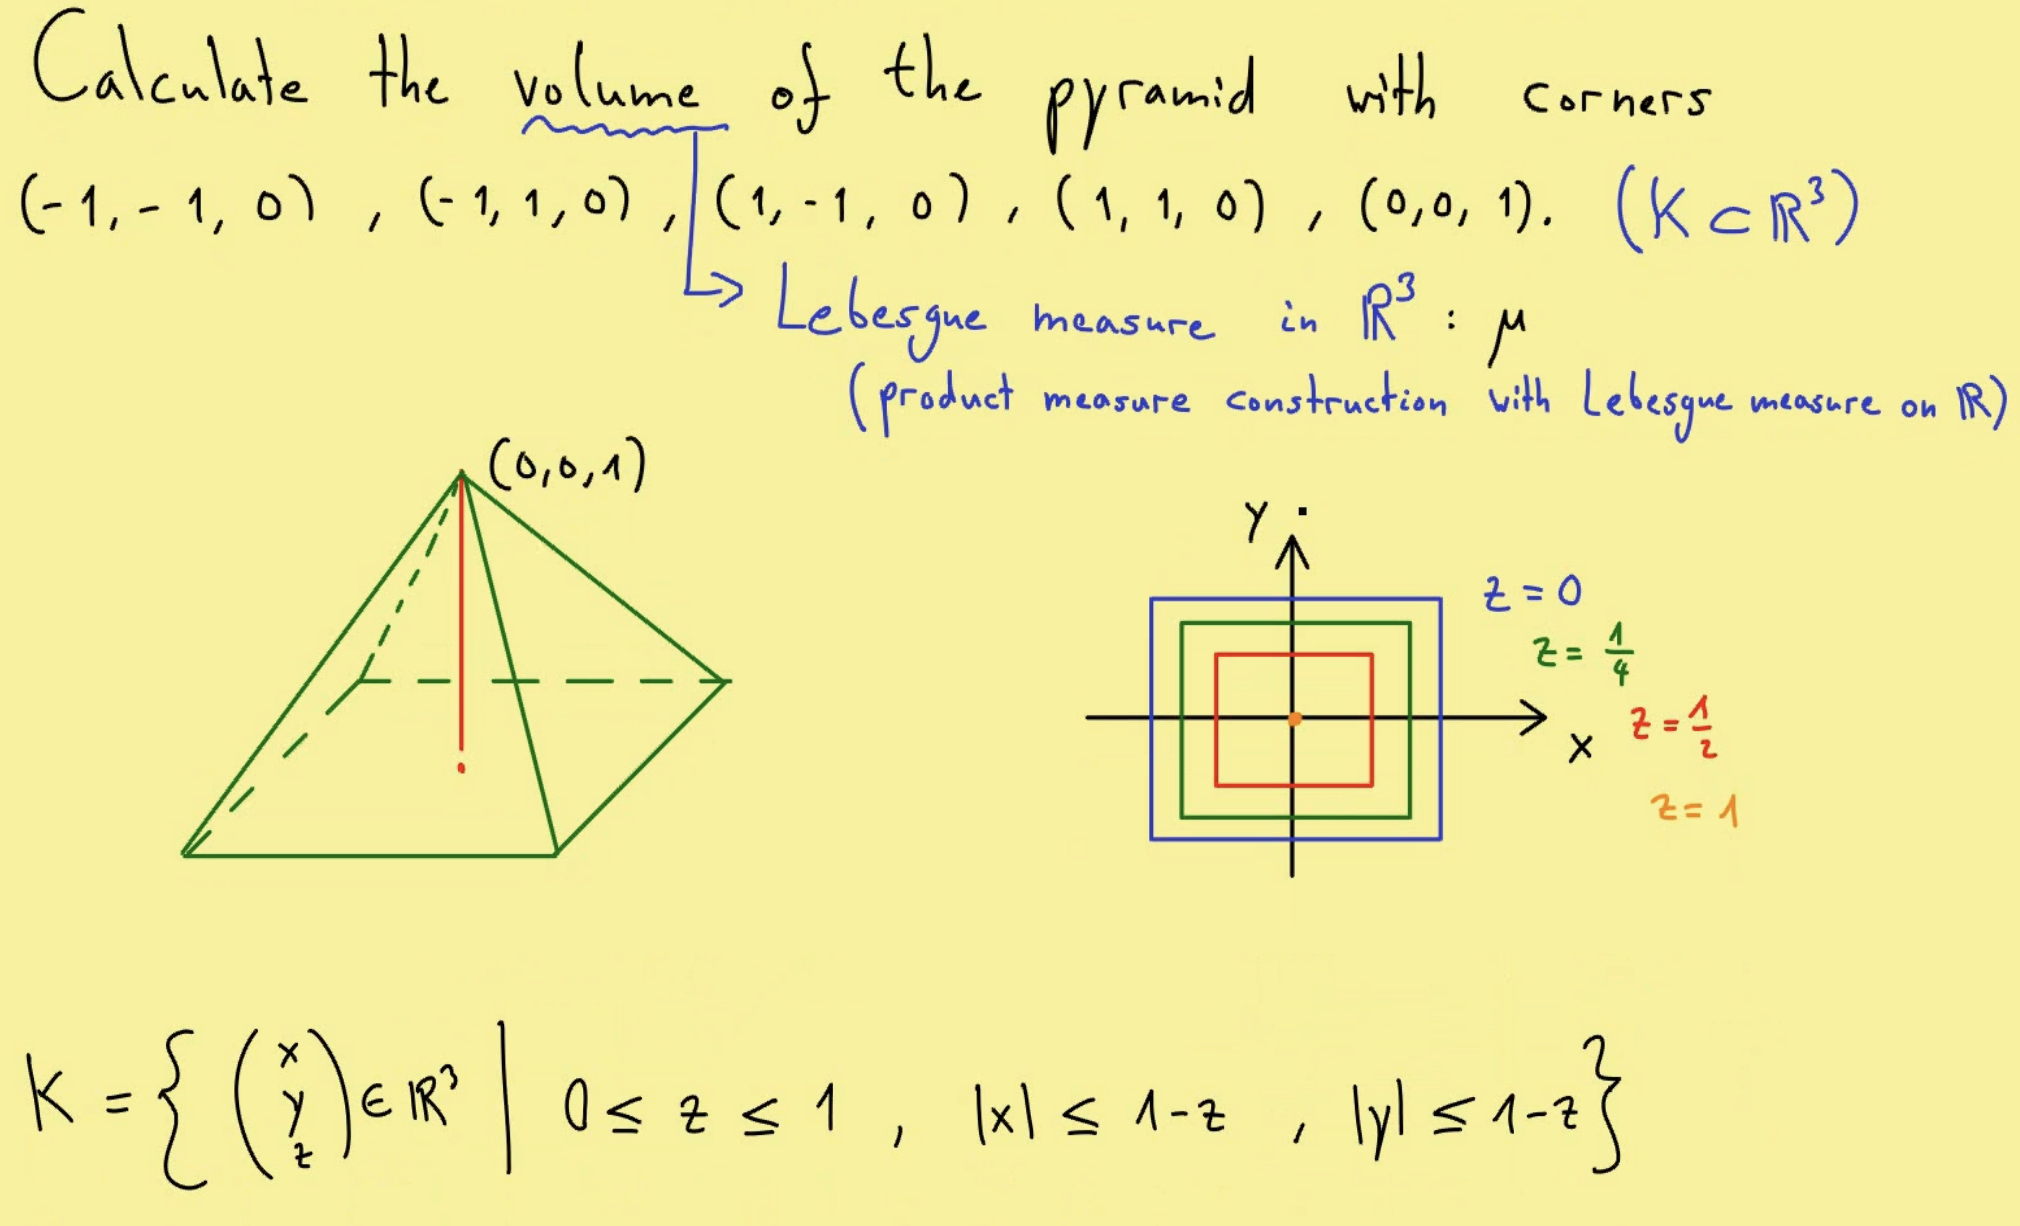
\includegraphics[scale=0.30]{../figures/pyramid.png}
    \begin{proof}
        Set
        \begin{align}
            K
            &= \left\{(x,y,z)^T \in \mathbb{R}^3 \vert 0 \leq z \leq 1, \vert x \vert \leq 1-z, \vert y \vert \leq 1-z \right\}.
        \end{align}
        Define $\mu$ as a product measure of $\mu_1$ and $\mu_2$, where $\mu_1$ is the lebesgue measure in $\mathbb{R}$(z-coordinate) and $\mu_2$ is the lebesgue measure on $\mathbb{R}^2$(x- and y-coordinate). Following the definition of product measure, we have the volume of $K$ as
        \begin{align}
            \mu(k)
            &= \int_{\mathbb{R}} \mu_2(M_{z_0})~{\rm d}\mu_1(z_0) \\
            &= \int_{[0,1]} 4 \cdot (1-z_0)^2{\rm d}\mu_1(z_0) \\
            &= \frac{4}{3},
        \end{align}
        where 
        \begin{align}
            M_{z_0}
            &:= \left\{(x,y)^T \in \mathbb{R}^2 \vert \vert x \vert \leq 1-z_0, \vert y \vert \leq 1-z_0 \right\},
        \end{align}
        and $\mu_2(M_{z_0})$ is the area of the square only for $z_0 \in [0,1]$.
    \end{proof}
\end{example}

\section{Fubini's theorem}
\begin{theorem}[Fubini's theorem]
    Let $\mu_1$ and $\mu_2$ be $\sigma$-finite, $\mu$ be the product measure and 
    \begin{align}
        f: X_1 \times X_2 \rightarrow [0,\infty]~measurable~[or~f \in \mathcal{L}^1(\mu)],
    \end{align}
    then:
    \begin{align}
        \int_{X_1 \times X_2} f~{\rm d}\mu
        &= \int_{X_2} \left(\int_{X_1} f(x,y)~{\rm d}\mu_1(x)\right)~{\rm d}\mu_2(x) \\
        &= \int_{X_1} \left(\int_{X_2} f(x,y)~{\rm d}\mu_2(x)\right)~{\rm d}\mu_1(x).
    \end{align}
\end{theorem}

\begin{example}
    $\mu$ lebesgue measure for $\mathbb{R}^2$. Calculate $\int_A f~{\rm d}\mu = ?$, where
    \begin{align}
        A
        &= \left\{(x,y)\in [0,1] \times [0,1] \vert x \geq y \geq x^2 \right\}, \\
        f(x,y)
        &= 2xy.
    \end{align}
    We have
    \begin{align}
        \int_A f~{\rm d}\mu
        &= \int_{\mathbb{R}^2} f\cdot \chi_A~{\rm d}\mu \\
        &= \int_{\mathbb{R}} \left(\int_{\mathbb{R}} f(x,y)\chi_A(x,y)~{\rm d}y\right)~{\rm d}x \\
        &= \int_0^1\left(\int_{x}^{x^2} 2xy~{\rm d}y\right)~{\rm d}x \\
        &= \frac{1}{12}.
    \end{align}
\end{example}

\section{Outer measure}
\begin{itemize}
    \item tools for the proof of (\ref{thm: caratheodory's extension theorem})
    \item "outer measure" is a new notion. "Outer measure" is not an attribute for "measure"! "Outer mesure" do not have to be measures!
\end{itemize}

\begin{definition}[Outer measure]
    \label{def: outer measure}
    A map $\phi: \mathcal{P}(X) \rightarrow [0,\infty]$ is called an outer measure if:
    \begin{itemize}
        \item (a) $\phi(\emptyset) = 0$
        \item (b) $A \subseteq B \Longrightarrow \phi(A) \leq \phi(B)$. (monotonicity)
        \item (c) $A_1, A_2,\dots, \in \mathcal{P}(X) \Longrightarrow \phi \left(\cup_{n=1}^\infty A_n \right) \leq \sum_{n=1}^{\infty} \phi(A_n)$. ($\sigma$-subadditivity)
    \end{itemize}
\end{definition}

\paragraph{Question:}
$\phi: \mathcal{P}(X) \rightarrow [0,\infty]$ outer measure $\stackrel{?}{\longrightarrow}$ $\mu$ measrue?

\begin{definition}[$\phi$-measurable]
    Let $\phi$ be an outer measure. $A \in \mathcal{P}(X)$ is called $\phi$-measurable if for all $Q \in \mathcal{P}(X)$ we have:
    \begin{align}
        \phi(Q)
        &\geq \phi(Q \cap A) + \phi(Q \cap A^c).
    \end{align}
\end{definition}

\begin{proposition}
    If $\phi: \mathcal{P}(X) \rightarrow [0,\infty]$ is an outer measure, then: 
    \begin{itemize}
        \item $\mathcal{A}_{\phi}:= \left\{A \subseteq X \vert A~\phi~measurable \right\}$ is a $\sigma$-algebra.
        \item $\mu: \mathcal{A}_{\phi} \rightarrow [0,\infty]$, $\mu(A) := \phi(A)$, is a measrue.
    \end{itemize}
\end{proposition}
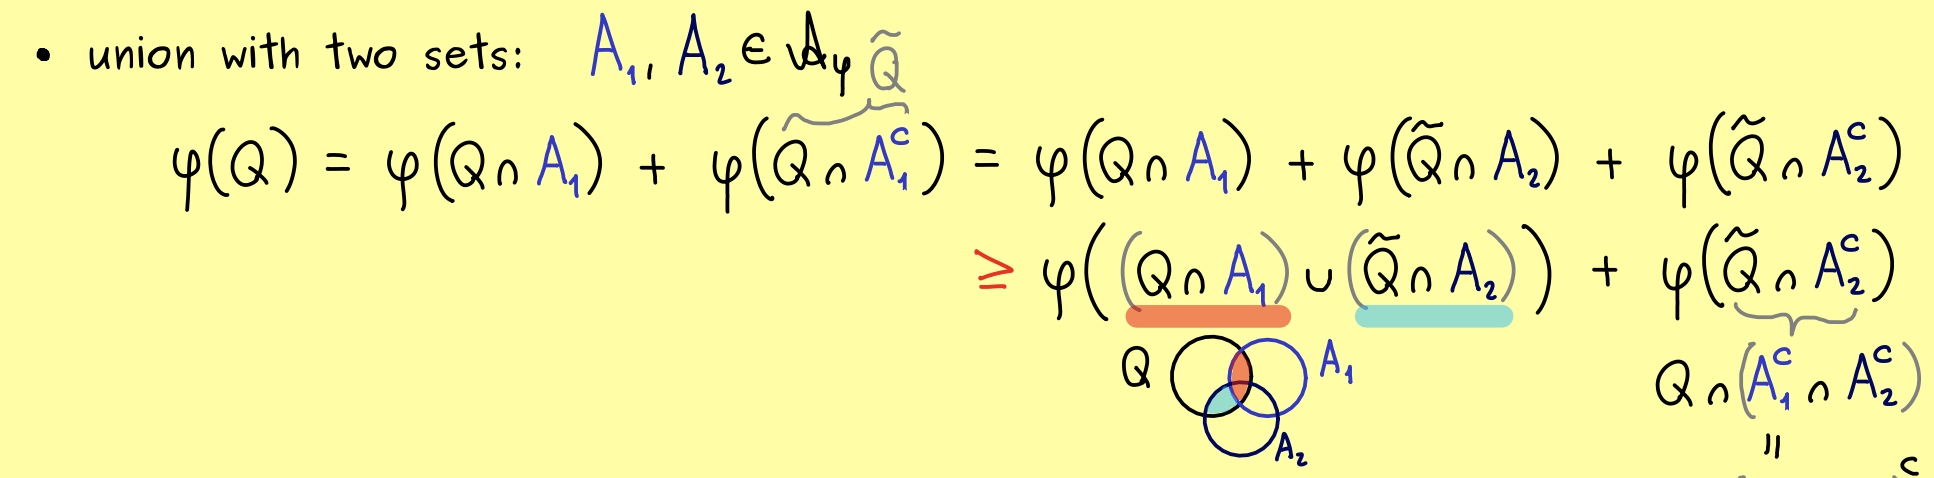
\includegraphics[scale=0.3]{../figures/pf trick of union case.png}
\begin{proof}
    \begin{itemize}
        \item $\phi \in \mathcal{A}_{\phi}$? Is $\emptyset$ $\phi$ -measurable? 
        \begin{align}
            \phi(Q)
            &= \phi(Q \cap \emptyset) + \phi(Q \cup \emptyset^c) \\
            &= 0+\phi(Q)
        \end{align}
        \item $X \in \mathcal{A}_{\phi}$? Is $X$ $\phi$-measurable? 
        \begin{align}
            \phi(Q)
            &= \phi(Q \cap X) + \phi(Q \cap X^c) \\
            &= \phi(Q) + \phi(\emptyset).
        \end{align}
        \item $A \in \mathcal{A}_{\phi} \Longrightarrow$
        \begin{align}
            \phi(Q)
            &= \phi(Q \cap A) + \phi(Q \cap A^c) \\
            &= \phi(Q \cap A^c) + \phi(Q \cap (A^c)^c) \\
            &\Longrightarrow A^c \in \mathcal{A}_{\phi}.
        \end{align} 
        \item union with two sets: $A_1, A_2 \in \mathcal{A}$ 
        \begin{align}
            \phi(Q)
            &= \phi(Q \cap A_1) + \phi(Q \cap A_1^c) \\
            &\qquad\eqnote{Define $\tilde{Q} := Q \cap A_1^c$} \nonumber \\
            &= \phi(Q \cap A_1) + \phi(\tilde{Q} \cap A_2) + \phi(\tilde{Q} \cap A_2^c) \\
            &\geq \phi\left((Q \cap A_1) \cup (\tilde{Q}\cap A_2)\right) + \phi(\tilde{Q} \cap A_2^c) \\
            &= \phi(Q \cap (A_1 \cup A_2)) + \phi(Q \cap (A_1 \cup A_2)^c),\\
            &\Longrightarrow \phi(Q) \geq \phi(Q \cap (A_1 \cup A_2)) + \phi(Q \cap (A_1 \cup A_2)^c) \\
            &\Longrightarrow A_1 \cup A_2 \in \mathcal{A}_{\phi},
        \end{align}
        where the fouth equation is obtain by the above figure.
        \item countable union: $A_1,A_2,\dots \in \mathcal{A}_{\phi}$, $A:= \cup_{j=1}^{\infty} A_j \in \mathcal{A}_{\phi}$?
        \begin{align}
            \phi(Q)
            &= \phi(Q \cap A_1) + \phi(Q \cap A_1^c) \\
            &\qquad\eqnote{Set $Q = \hat{Q}\cap (A_1 \cup A_2)$} \nonumber \\
            &= \phi(\hat{Q}\cap A_1) + \phi(\hat{Q}\cap A_2).
        \end{align}
        Induction: $\phi(\hat{Q}\cap \cup_{j=1}^{n} A_j) = \sum_{j=1}^{n} \phi(\hat{Q} \cap A_j)$.
        We have:
        \begin{align}
            \phi(\hat{Q})
            &= \phi(\hat{Q}\cap \cup_{j=1}^{n}) + \phi(\hat{Q} \cap (\cup_{j=1}^n A_j)^c) \\
            &\geq \sum_{j=1}^n \phi(\hat{Q}\cap A_j) + \phi(\hat{Q}\cap A^c) \\
            \Longrightarrow \phi(\hat{Q}) 
            &\geq \sum_{j=1}^n \phi(\hat{Q}\cap A_j) + \phi(\hat{Q}\cap A^c) \\
            &\geq \phi(\hat{Q} \cap A) + \phi(\hat{Q} \cap A^c) \\
            &\geq \phi(\hat{Q}) \\
            &\Longrightarrow A \in \mathcal{A}_{\phi}.
        \end{align}
    \end{itemize}
\end{proof}

\begin{example}
    (1) $\phi:\mathcal{P}(\mathbb{R}) \rightarrow [0,\infty]$,
    \begin{align}
        \phi(A)
        &= \left\{
            \begin{matrix}
                0,&~A = \emptyset \\
                1,&~A \neq \emptyset.
            \end{matrix}
        \right.
        &\Longrightarrow outer~measure~but~not~a~measure!
    \end{align}
\end{example}

\begin{example}
    $\phi: \mathcal{P}(\mathbb{N}) \rightarrow [0,\infty]$, 
    \begin{align}
        \phi(A)
        &= \left\{
            \begin{matrix}
                \vert A \vert,&~A~finite \\
                \infty,&~A~not~finite.\\
            \end{matrix}
        \right\}\\
        &\Longrightarrow outer~measure~but~a~measure!(counting~measure)
    \end{align}
\end{example}

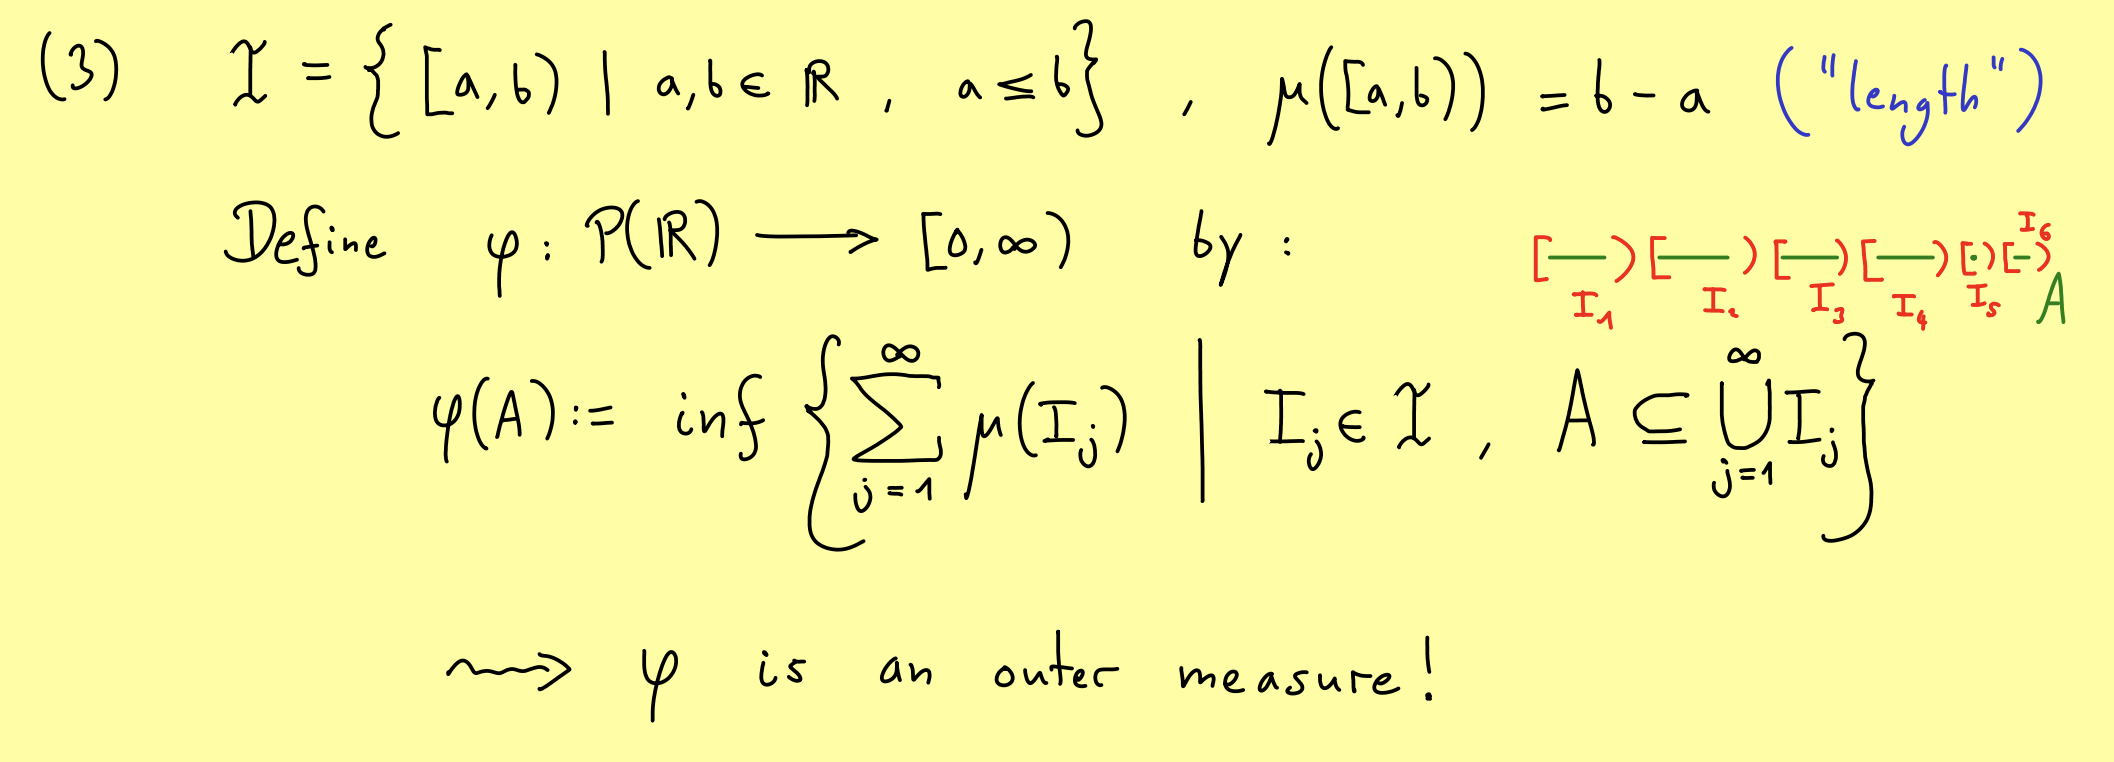
\includegraphics[scale = 0.3]{../figures/outer measure.png}
\begin{example}
    $\mathcal{I} = \left\{[a,b) \vert a,b \in \mathbb{R},~a \leq b\right\}$, $\mu([a,b)) = b-a$("length").

    Define $\phi: \mathcal{P}(\mathbb{R}) \rightarrow [0,\infty)$ by:
    \begin{align}
        \phi(A)
        &:= \inf\left\{\sum_{j=1}^{\infty} \mu(I_j) \vert I_j \in \mathcal{I},~A \subseteq \cup_{j=1}^{\infty} I_j \right. \\
        &\Longrightarrow \phi~is~an~outer~measure!
    \end{align}
    \begin{proof}
        check (a) of (\ref{def: outer measure}): $\phi(\emptyset) = 0$.

        check (b) of (\ref{def: outer measure}): monotonicity, 
        \begin{align}
            A \subseteq B 
            &\Longrightarrow \phi(B) \\
            &= \inf\left\{\sum_{j=1}^{\infty} \mu(I_j) \vert I_j \in \mathcal{I},~B \subseteq U_{j=1}^{\infty} I_j \right\} \\
            & \geq \inf\left\{\sum_{j=1}^{\infty} \mu(I_j) \vert I_j \in \mathcal{I},~A \subseteq U_{j=1}^{\infty} I_j \right\},
        \end{align}
        since $A \subseteq B$.

        check (c) of (\ref{def: outer measure}): show that $\phi(\cup_{n \in \mathbb{N}}A_n) \leq \sum_{n \in \mathbb{N}} \phi(A_n)$. Let $\varepsilon > 0$. Choose $\varepsilon_n > 0 $ with $\sum_{n \in \mathbb{N}} \varepsilon_n = \varepsilon$. Then there are intervals $I_{j,n}$ with:
        \begin{align}
            \phi(A_n)
            &\geq \sum_{j=1}^{\infty} \mu(I_{j,n}) - \varepsilon_n,
        \end{align}
        and
        \begin{align}
            A_n \subseteq \cup_{j=1}^{\infty} I_{j,n}.
        \end{align}
        Then: $\cup_{n \in \mathbb{N}} \subseteq \cup_{n \in \mathbb{N}} \cup_{j \in \mathbb{N}} I_{j,n} = \cup_{j,n} I_{j,n}$.
        \begin{align}
            \Longrightarrow \phi(\cup_{n \in \mathbb{N}}) 
            &\stackrel{(b)}{\leq} \phi(\cup_{j,n} I_{j,n}) \\
            &\leq \sum_{j,n} \mu(I_{j,n}) \\
            &= \sum_{n \in \mathbb{N}} \left\{\sum_{j \in \mathbb{N}} \mu(I_{j,n})\right\} \\
            &\leq \sum_{n \in \mathbb{N}}\left(\phi(A_n)+\varepsilon_n \right) \\
            &= \sum_{n \in \mathbb{N}} \phi(A_n) + \varepsilon.
        \end{align}
    \end{proof}
\end{example}



\end{document}